% Created 2019-04-15 Mon 14:15
% Intended LaTeX compiler: pdflatex
\documentclass[11pt]{article}
\usepackage[utf8]{inputenc}
\usepackage[T1]{fontenc}
\usepackage{graphicx}
\usepackage{grffile}
\usepackage{longtable}
\usepackage{wrapfig}
\usepackage{rotating}
\usepackage[normalem]{ulem}
\usepackage{amsmath}
\usepackage{textcomp}
\usepackage{amssymb}
\usepackage{capt-of}
\usepackage{hyperref}
\usepackage{minted}
\usepackage[a4paper, margin=2cm]{geometry}
\usepackage{indentfirst}
\usepackage[, brazilian]{babel}
\usepackage{float}
\usepackage{color, colortbl}
\usepackage{titling}
\setlength{\droptitle}{-1.5cm}
\hypersetup{ colorlinks = true, urlcolor = blue }
\usemintedstyle{murphy}
\definecolor{beige}{rgb}{0.93,0.93,0.82}
\definecolor{brown}{rgb}{0.4,0.2,0.0}
\author{Fernanda Guimarães - 2016058166}
\date{}
\title{Exercício 06 - (entrega 15/04)}
\hypersetup{
 pdfauthor={Fernanda Guimarães - 2016058166},
 pdftitle={Exercício 06 - (entrega 15/04)},
 pdfkeywords={},
 pdfsubject={},
 pdfcreator={Emacs 26.1 (Org mode 9.2)},
 pdflang={Brazilian}}
\begin{document}

\maketitle

\section{Q1}
\label{sec:orgda2c960}
\begin{figure}[H]
\centering
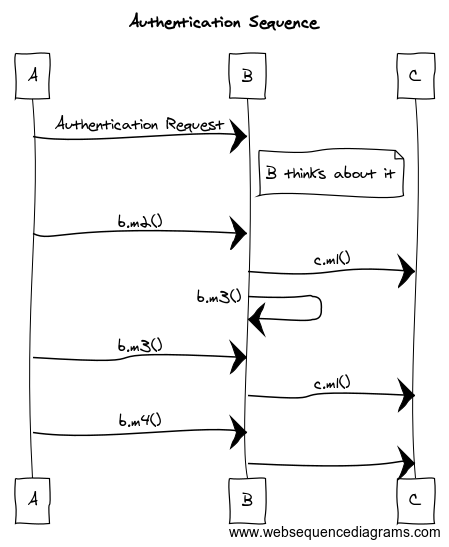
\includegraphics[height=200px]{./sequence.png}
\caption{Diagrama de Sequência}
\end{figure}

\section{Q2 \& Q3}
\label{sec:orge563db5}
\url{https://github.com/haneybarg-es/DesignPatterns}
\end{document}
